% --------------------------------------------------------------
% This is all preamble stuff that you don't have to worry about.
% Head down to where it says "Start here"
% --------------------------------------------------------------
 
\documentclass[12pt]{article}
 
\usepackage[margin=1in]{geometry} 
\usepackage{amsmath,amsthm,amssymb}
\usepackage{gensymb}
\usepackage{graphicx}
 \usepackage{tikz,pgfplots}
\usepackage{float}
\usepackage{enumitem}
\usepackage[utf8]{inputenc}


\newcommand{\N}{\mathbb{N}}
\newcommand{\Z}{\mathbb{Z}}

\newcommand{\slantedgrid}[4]{%
   \pgfmathtruncatemacro{\result}{#1+#3}
   \foreach \x in {#1,...,\result} \draw (\x,#2) -- ++(#4,#4);%
   \pgfmathtruncatemacro{\result}{#2+#4}
   \foreach \y in {#2,...,\result} \draw (#1+\y-#2,\y) -- ++(#3,0);%
 }
 
\DeclareMathOperator\erf{erf}
 
\newenvironment{theorem}[2][Theorem]{\begin{trivlist}
\item[\hskip \labelsep {\bfseries #1}\hskip \labelsep {\bfseries #2.}]}{\end{trivlist}}
\newenvironment{lemma}[2][Lemma]{\begin{trivlist}
\item[\hskip \labelsep {\bfseries #1}\hskip \labelsep {\bfseries #2.}]}{\end{trivlist}}
\newenvironment{exercise}[2][Exercise]{\begin{trivlist}
\item[\hskip \labelsep {\bfseries #1}\hskip \labelsep {\bfseries #2.}]}{\end{trivlist}}
\newenvironment{problem}[2][Problem]{\begin{trivlist}
\item[\hskip \labelsep {\bfseries #1}\hskip \labelsep {\bfseries #2.}]}{\end{trivlist}}
\newenvironment{question}[2][Question]{\begin{trivlist}
\item[\hskip \labelsep {\bfseries #1}\hskip \labelsep {\bfseries #2.}]}{\end{trivlist}}
\newenvironment{corollary}[2][Corollary]{\begin{trivlist}
\item[\hskip \labelsep {\bfseries #1}\hskip \labelsep {\bfseries #2.}]}{\end{trivlist}}
 
\begin{document}
\providecommand{\e}[1]{\ensuremath{\times 10^{#1}}}
\providecommand{\ex}[1]{\ensuremath{10^{#1}}}
% --------------------------------------------------------------
%                         Start here
% --------------------------------------------------------------
 
\title{HW 7}
\author{Levon Dovlatyan \\ SI: 24451582\\ E45} 
\date{Oct 31, 2014}
\maketitle
 
\begin{problem}{10.1} 
For an aluminum alloy, the activation energy for crystal growth is 120 kJ/mol.  By what factor would the rate of crystal growth change by dropping the alloy temperature from 500$\degree$C to room temperature (25$\degree$C)?
\end{problem}
Let $T_1 = 500\degree$C and $T_2 = 25\degree$C. Activation energy $Q = 120$kJ and the gas constant $k = 8.314$J/(mol*K).
\begin{align*}
&\frac{\dot{G_1} = Ce^{\frac{-Q}{RT_1}}}{\dot{G_2} = Ce^{\frac{-Q}{RT_2}}} \Rightarrow \frac{\dot{G_1} = e^{\frac{Q}{kT_2}}}{\dot{G_2} = e^{\frac{Q}{kT_1}}} \Rightarrow \frac{\dot{G_1}}{\dot{G_2}} = e^{\frac{Q}{R}(\frac{1}{T_2}-\frac{1}{T_1})} \Rightarrow \dot{G_1} = \dot{G_2}e^{\frac{Q}{R}(\frac{1}{T_2}-\frac{1}{T_1})}  \\\\  \dot{G_1} &= \dot{G_2}e^{\frac{Q}{R}(\frac{1}{T_2}-\frac{1}{T_1})} \Rightarrow \dot{G_1} = \dot{G_2}e^{\frac{120000}{8.314}(\frac{1}{25+273}-\frac{1}{500+273})} \Rightarrow \dot{G_1} = 8.43\e{12}\dot{G_2}
\end{align*}

\begin{problem}{10.11}
(a)  A carbon steel with 1.13 wt\% C is given the following heat treatment: (i) instantaneously quenched to 200$\degree$C, (ii) held for 1 day, and (iii) cooled slowly to room temperature.  What is the resulting microstructure? \textbf{(b)} What microstructure would result if a carbon steel with 0.5 wt\% C were given exactly the same heat treatment?
\end{problem}

\textbf{(a)} Since the temperature is held at 200$\degree$C, the steel does not enter the martensite region, instead it stays on the border between bainite and martenite. Now at 1 day, the steel is fully in the Bainite region since it is at the solidification temperature. This means the steel microstructure must be 100\% Bainite.

\textbf{(b)} Looking at Figure 10.16 in the book [1], we can see that a temperature of 200$\degree$ is near the 90\% martensite line. So our sample will contain 90\% martensite and obtain 10\% of the original austenite.

\begin{problem}{10.21}
It is worth noting that in TTT diagrams such as Figure 10.7, the 50\% completion (dashed line) curve lies roughly midway between the onset (1\%) curve and completion (99\%) curve.  It is also worth noting that the progress of transformation is not linear, but instead is sigmoidal (s-shaped) in nature.  For example, careful observation of Figure 10.7 at 500$\degree$C show that 1\%, 50\%, and 99\% completion occur at 0.9 s, 3.0 s, and 9.0 s, respectively.  Intermediate completion data, however, can be given as follows: \\
\begin{center}
\begin{tabular}{c | c}
\% \textbf{completion} & \textbf{t(s)} \\
20 & 2.3 \\
40 & 2.9 \\
60 & 3.2 \\
80 & 3.8 \\
\end{tabular}
\end{center}
Plot the \% completion at 500$\degree$C versus log t to illustrate the sigmoidal nature of the transformation.
\end{problem}

\begin{figure}[H]
\centering
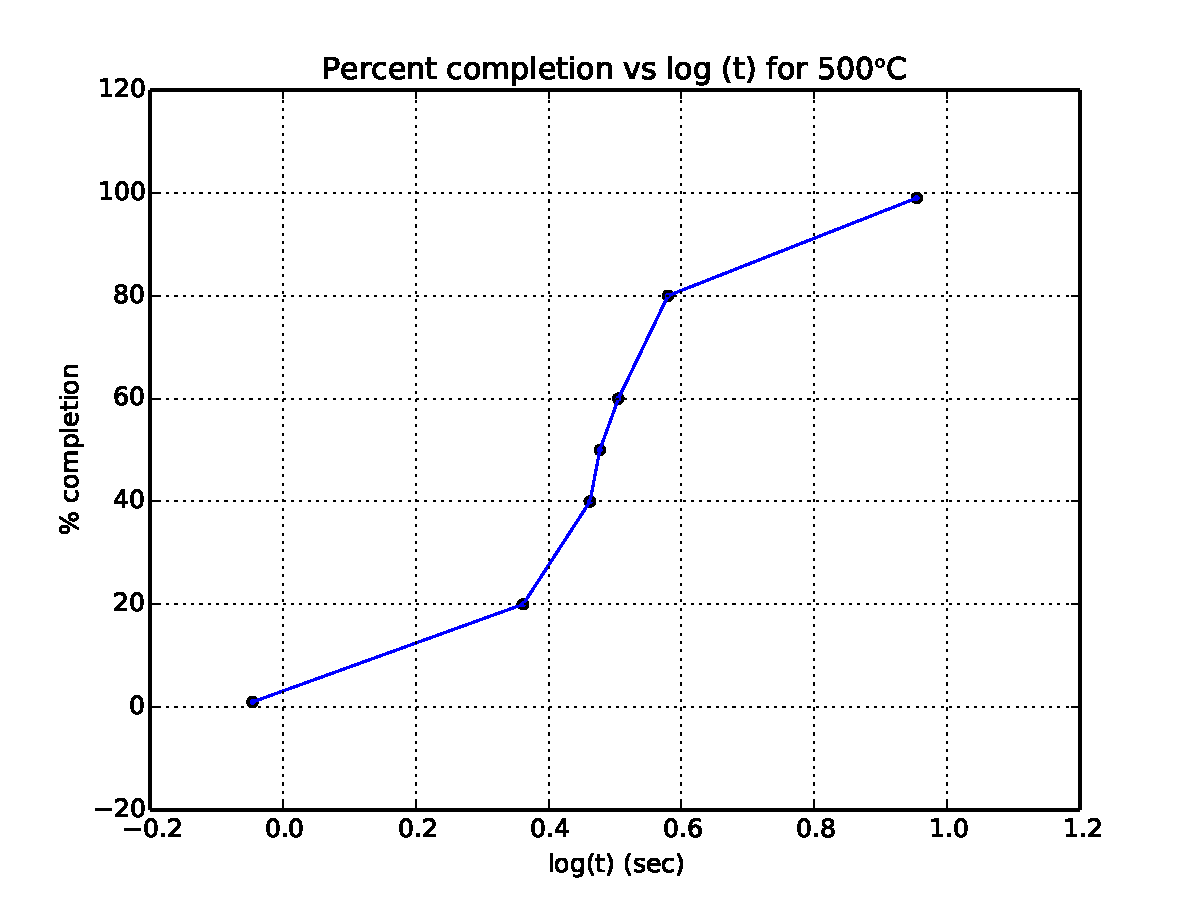
\includegraphics[width=300pt]{graphs/p21.pdf}
\caption{}
\end{figure}

\begin{problem}{10.31}
 In heat-treating a complex-shaped part made from a 5140 steel, a final quench in stirred oil leads to a hardness of Rockwell C30 at 3 mm beneath the surface.  This hardness is unacceptable, as design specifications require a hardness of Rockwell C45 at that point.  Select an alloy substitution to provide this hardness, assuming the heat treatment must remain the same.
 \end{problem}
 
 Looking at Fig 10.24 in the book [1], A rockwell C value of 30 corresponds to 10/16 inch for the quench distance of 5140. According to the problem, we want to pick a material that has this same quench distance, 10/16 inch, but offers us atleast a rockwell hardness of C45. The only two alloys that have a rockwell C value of 45 or great when the quench distance is 10/16 inch are 4340 and 9840 Steel.
 
 \begin{problem}{10.41}
 Recrystallization is a thermally activated process and, as such, can be characterized by the Arrhenius expression (Equation 5.1). As a first approximation, we can treat ${t_R}^{–1}$ as a “rate,” where $t_R$ is the time necessary to fully recrystallize the microstructure.  For a 75\% cold-worked aluminum alloy, $t_R$ is 100 hours at 250$\degree$C and only 10 hours at 280$\degree$C.  Calculate the activation energy for this recrystallization process. (Note Problem 10.35, in which a similar method was applied to the case of precipitation hardening.)
 \end{problem}
 
 Given that $t_R1 = 100$ hours, $t_R2 = 10$ hours, $T_1 = 250\degree$C, and $T_2 = 280\degree$C, we can solve this problem the same way we did for problem 1 in this hw.
 
 \begin{align*}
 &\frac{{t_{R1}}^{-1}}{{t_{R2}}^{-1}} = \frac{Ce^{\frac{-Q}{RT_1}}}{Ce^{\frac{-Q}{RT_2}}} \Rightarrow \frac{\frac{1}{100}}{\frac{1}{10}} = \frac{e^{\frac{Q}{RT_2}}}{e^{\frac{Q}{RT_1}}} \Rightarrow \frac{1}{10} = e^{\frac{Q}{R}(\frac{1}{T_2}-\frac{1}{T_1})} \Rightarrow \ln{0.1} = \frac{Q}{R}(\frac{1}{T_2}-\frac{1}{T_1}) \\\\ & \ln{0.1} = \frac{Q}{R}(\frac{1}{T_2}-\frac{1}{T_1}) \Rightarrow Q = \frac{RT_1T_2\ln{0.1}}{T_1 - T_2} \Rightarrow Q = \frac{(8.314)(\ln{0.1})(523)(553)}{523 - 553} = 185\text{kJ}
 \end{align*}

\section{References}
\begin{enumerate}
\item James F. Shackelford, Introduction to Materials Science for Engineers, Seventh Edition, Pearson Higher Education, Inc., Upper Saddle River, New Jersey (2009).
\end{enumerate}




% --------------------------------------------------------------
%     You don't have to mess with anything below this line.
% --------------------------------------------------------------
 
\end{document}
